% !TEX TS-program = xelatex
% !TEX encoding = UTF-8 Unicode

\documentclass[a4paper,11pt]{article}
\usepackage{xeCJK}
\setCJKmainfont{IPAexMincho}
\setCJKsansfont{IPAexGothic}
\setCJKmonofont{IPAexGothic}
\usepackage[a4paper,margin=25mm]{geometry}
\usepackage{parskip}               % 段落間の余白
\setlength{\parindent}{0pt}        % 行頭インデントなし
\usepackage{enumitem}
\setlist[itemize,1]{label=・, left=0pt, nosep}
\usepackage{titlesec}
\usepackage{listings}
\usepackage{xcolor}
\usepackage[dvipdfmx]{graphicx}
\usepackage{float}


\lstset{
  language=Python,
  basicstyle=\ttfamily\small,
  breaklines=true,
  columns=fullflexible,
  inputencoding=utf8,
  keywordstyle=\color{blue},
  commentstyle=\color{gray},
  stringstyle=\color{teal},
  showstringspaces=false,
}
\titlespacing*{\subsection}{0pt}{9ex}{1ex}

\begin{document}

%―――――――――――――――――――――――――――――――――――――――
% タイトルブロック
\begin{center}
  {\LARGE \bfseries ウェアラブル端末と心理入力アプリデータを統合した\\感情予測アルゴリズムの開発}\\[6ex]
\end{center}

\hrule\vspace{1ex}
{\normalsize 2025-06-13 進捗報告 \hfill 森雄大}\\
\hrule\vspace{5ex}



%―――――――――――――――――――――――――――――――――――――――
% データ収集・解析の概要
\subsection*{感情スコアの時間傾向}
線形混合モデル(Linear Mixed Model, LMM)を使い、目的変数である感情スコアを固定効果とランダム効果で説明するモデルを構築した。

\vspace{2ex}
\noindent \textbf{【データ構造】}

感情スコアデータ一つ一つに、計測した時間帯カテゴリ(例:00:00–03:00)と被験者IDを紐づけ、データを被験者グループ単位で扱えるようにした。

\vspace{2ex}
\noindent \textbf{【モデル構造】}

\begin{itemize}
\item 固定効果:全被験者に共通した時間帯カテゴリの効果
\item ランダム効果:被験者ごとのベースラインの個人差
\end{itemize}

\vspace{2ex}
\noindent \textbf{【結果の解釈】}

\begin{itemize}
\item 固定効果:被験者個人差を除いた時間帯別の平均的なArousal・Valenceスコア
\item ランダム効果の分散:被験者間のベースラインの個人差の程度
\end{itemize}

arousal ~ 1 + timeBin + (1|subjectId)

valence ~ 1 + timeBin + (1|subjectId)


\subsection*{感情スコアの可視化}
時間帯による感情スコアの傾向を追うため、全感情計測データを時間帯カテゴリ別にプロットした(図1・2)。

\vspace{1ex}
\noindent \textbf{【注意】} 感情スコアが0–10の整数値のため、データポイントが重ならないよう±0.5 のジッタリングを適用している。

\begin{figure}[H]
  \centering
  \begin{minipage}{0.4\columnwidth}
     \centering
     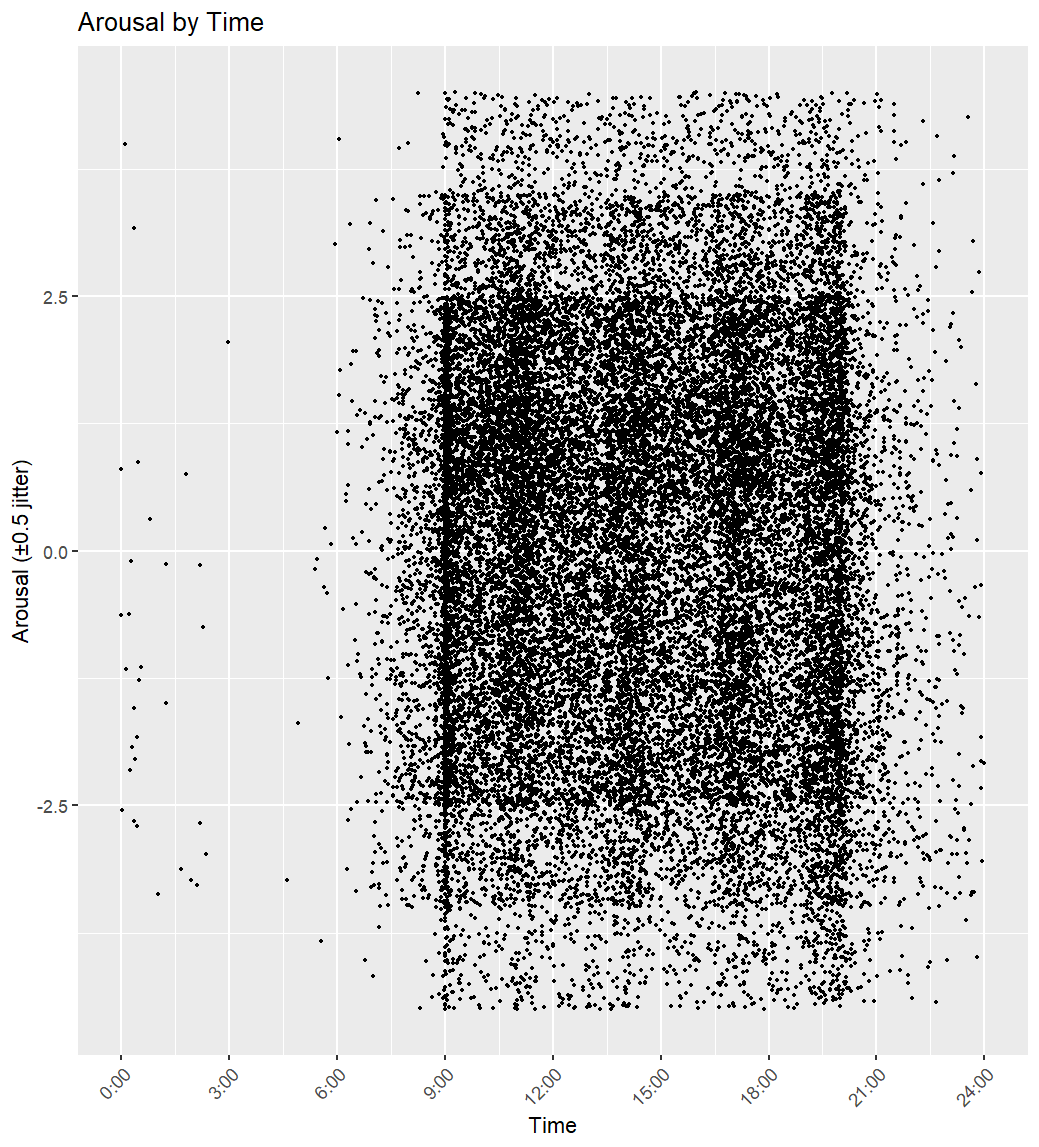
\includegraphics[width=\columnwidth]{/home/mori/projects/affective-forecast/R-workspace/arousal_by_time.png}
     \caption{Arousalの時間帯カテゴリ別分布(ジッタあり)\\y軸:Arousalスコア(0–10の整数値に±0.5ジッタ適用)}
  \end{minipage}
%
  \begin{minipage}{0.4\columnwidth}
     \centering
     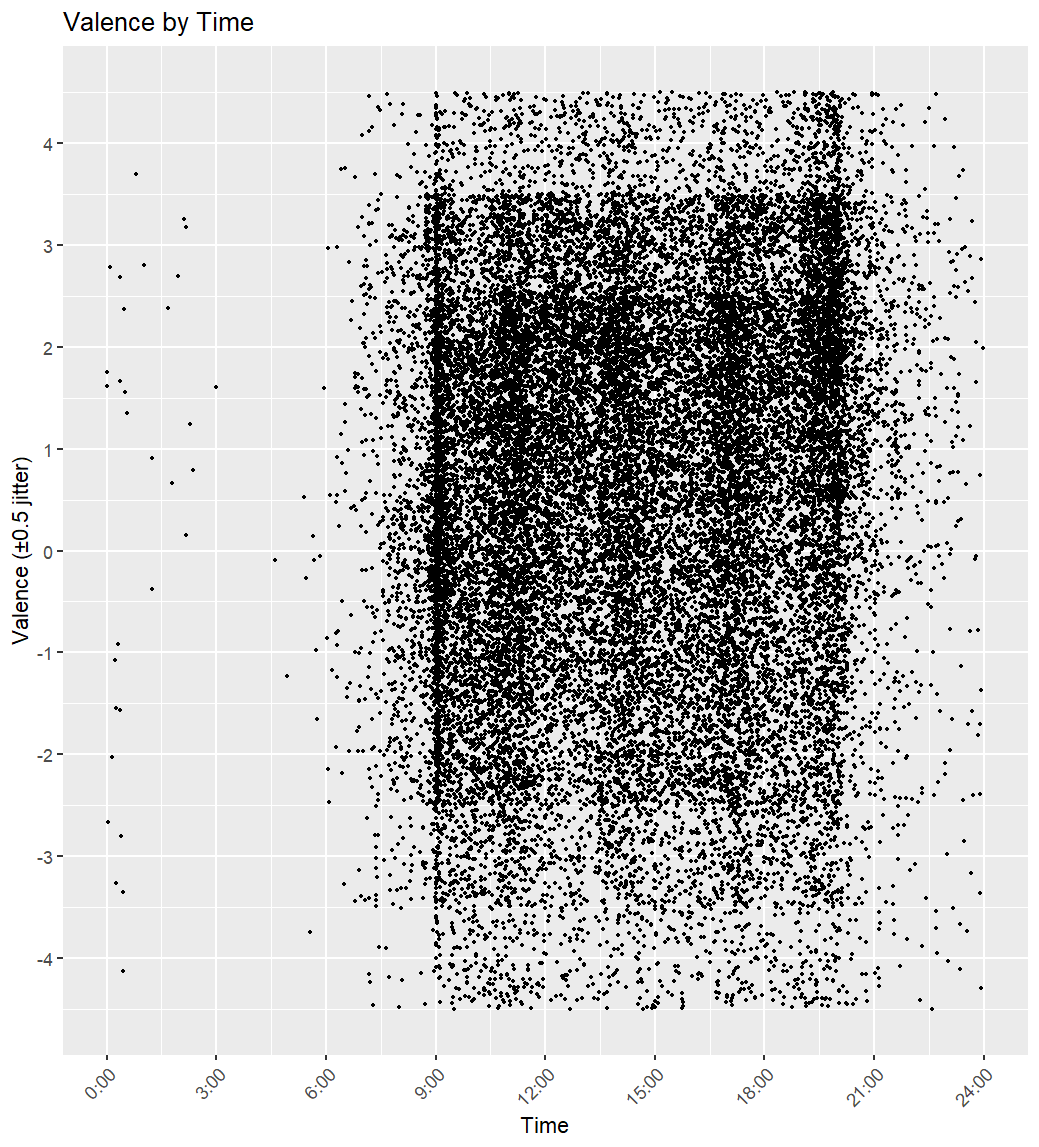
\includegraphics[width=\columnwidth]{/home/mori/projects/affective-forecast/R-workspace/valence_by_time.png}
     \caption{Valenceの時間帯カテゴリ別分布(ジッタあり)\\y軸:Valenceスコア(0–10の整数値に±0.5ジッタ適用)}
  \end{minipage}
\end{figure}

\subsection*{感情スコアの固定効果の可視化}
線形混合モデルで推定した固定効果(時間帯別の推定平均値)とその標準誤差を以下に示す(図3・4)。

\vspace{1ex}
\noindent \textbf{【読み方】} エラーバーは95%信頼区間を表し、バーが重ならない時間帯間には有意差がある可能性が高い。

\begin{figure}[H]
  \centering
  \begin{minipage}{0.4\columnwidth}
     \centering
     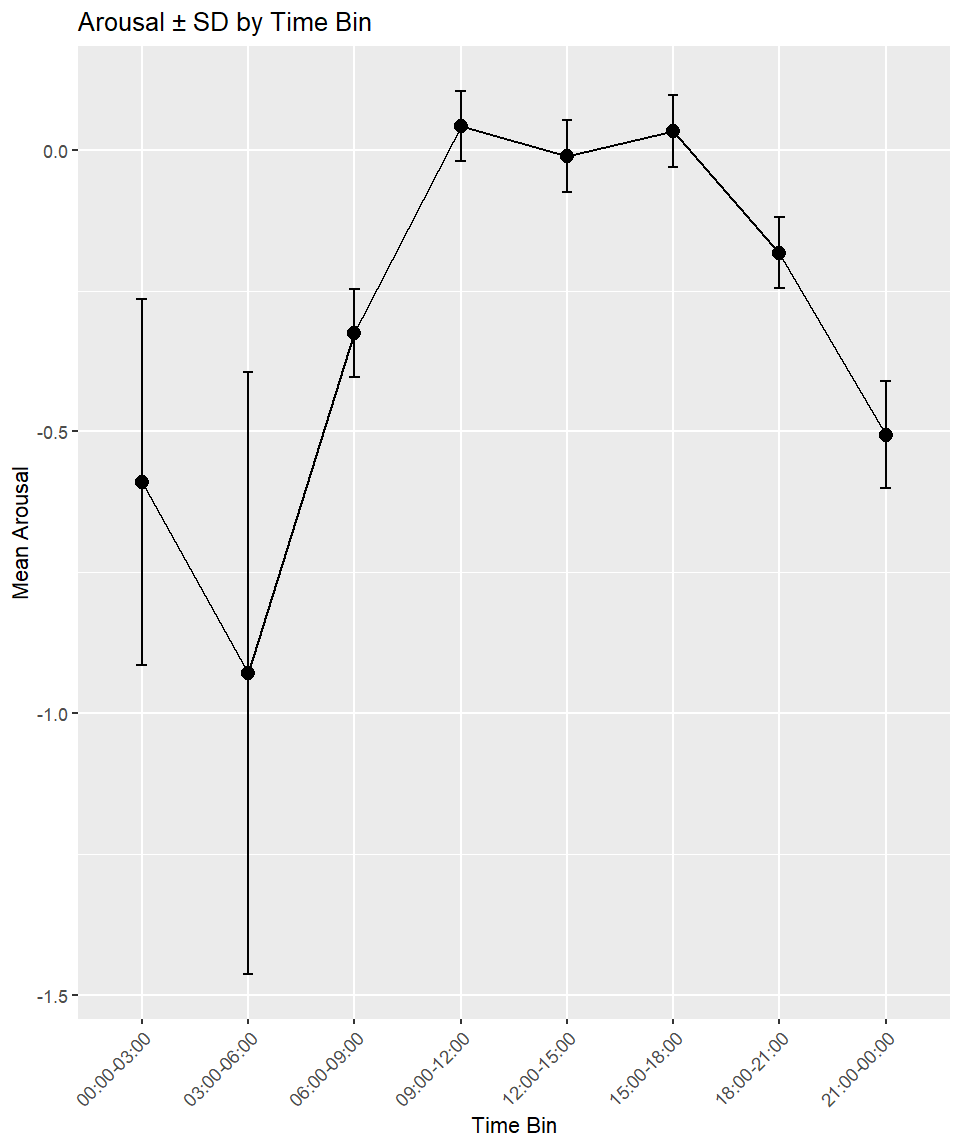
\includegraphics[width=\columnwidth]{/home/mori/projects/affective-forecast/R-workspace/arousal_by_timebin.png}
     \caption{時間帯別 Arousal の推定平均値(固定効果)および標準誤差(SE)}
  \end{minipage}
%
  \begin{minipage}{0.4\columnwidth}
     \centering
     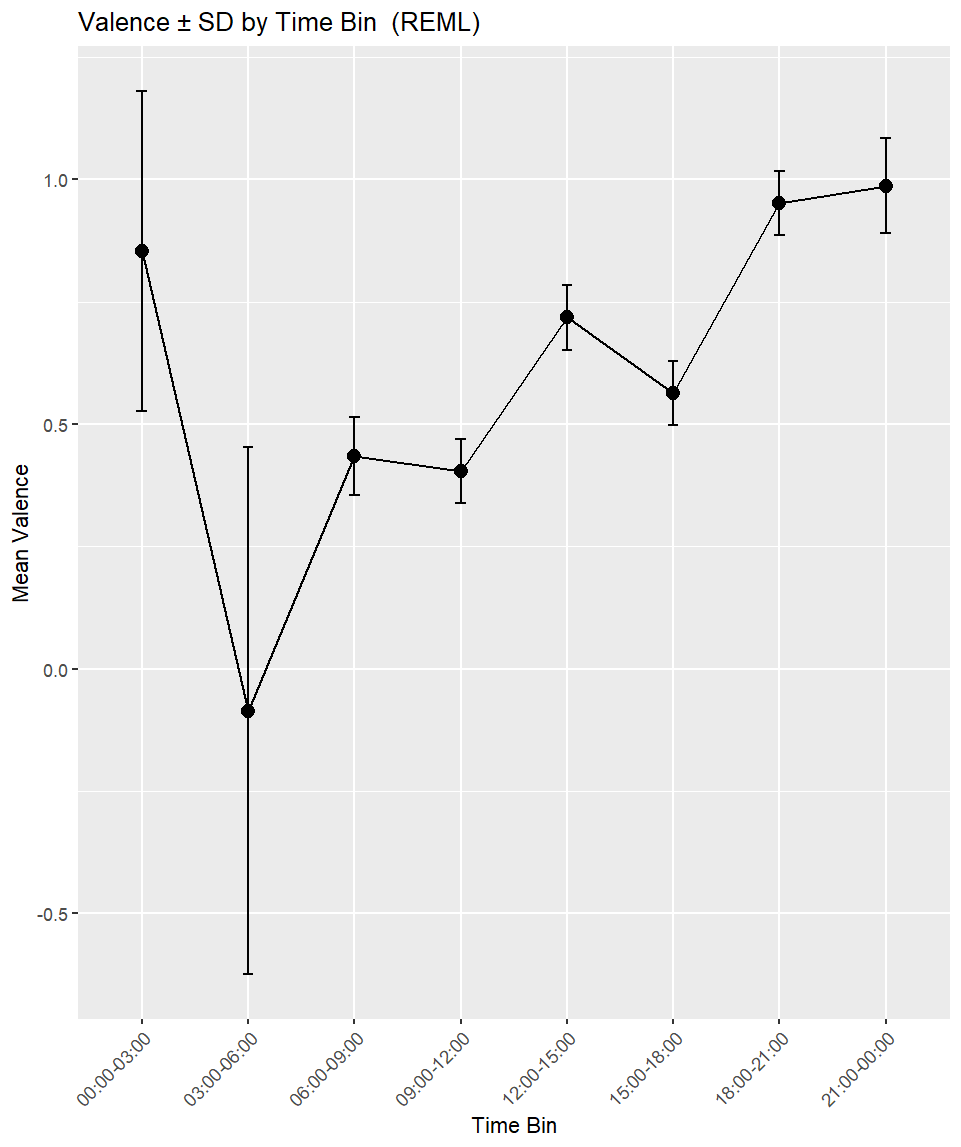
\includegraphics[width=\columnwidth]{/home/mori/projects/affective-forecast/R-workspace/valence_by_timebin.png}
     \caption{時間帯別 Valence の推定平均値(固定効果)および標準誤差(SE)}
  \end{minipage}
\end{figure}


\subsection*{その他メタデータをカテゴリ変数として考慮}
基本モデルでは時間帯のみを説明変数としていたが、被験者の個人特性(メタデータ)を追加することで、より精度の高い推定が可能か検討した。

\vspace{2ex}
\noindent \textbf{【追加したメタデータ】}

\begin{itemize}
\item 性別(男性・女性)

\item 年齢(10歳単位でカテゴリ化)

\item 楽観性(質問票の楽観的設問に対する平均スコアを四捨五入で1~4の整数化)

\item 悲観性(質問票の悲観的設問に対する平均スコアを四捨五入で1~4の整数化)

\end{itemize}

\vspace{2ex}
以下に、各メタデータを考慮したモデルの推定結果を示す。

\vspace{3ex}
\subsection*{モデル比較による効果の検証}

各メタデータを追加したモデルの性能をAIC(Akaike Information Criterion)で比較した。AICが小さいほど良いモデルであり、ベースモデル(①)からのΔAICで改善度を評価した。

\vspace{2ex}
\begin{table}[H]
\centering
\begin{tabular}{|c|l|r|r|r|r|}
\hline
モデル & 固定効果の追加 & AIC (arousal) & ΔAIC vs ① & AIC (valence) & ΔAIC vs ① \\
\hline
① & time\_bin & \textbf{115,599.8} & 0.0 & \textbf{116,106.1} & 0.0 \\
② & + gender & 115,601.7 & +1.9 & \textbf{116,103.0} & \textbf{−3.1} \\
③ & + age & 115,605.5 & +5.7 & 116,111.7 & +5.6 \\
④ & + mean\_optimism & 115,601.9 & +2.1 & 116,107.0 & +0.9 \\
⑤ & + mean\_pessimism & 115,604.9 & +5.1 & 116,110.4 & +4.3 \\
\hline
\end{tabular}
\caption{各メタデータを追加したモデルのAIC比較}
\end{table}

\vspace{2ex}
\noindent \textbf{【要点】}

\begin{itemize}
\item \textbf{valence}は②(+gender)でのみAICが有意に改善(−3.1)
\item それ以外はAICが上昇または微増で、情報量的には\textbf{追加メリットなし}
\item arousalについては、すべてのメタデータ追加でAICが悪化
\item 性別のみがvalence推定に有効な追加情報を提供
\end{itemize}

\vspace{3ex}
\subsubsection*{性別による効果}
\begin{figure}[H]
  \centering
  \begin{minipage}{0.4\columnwidth}
     \centering
     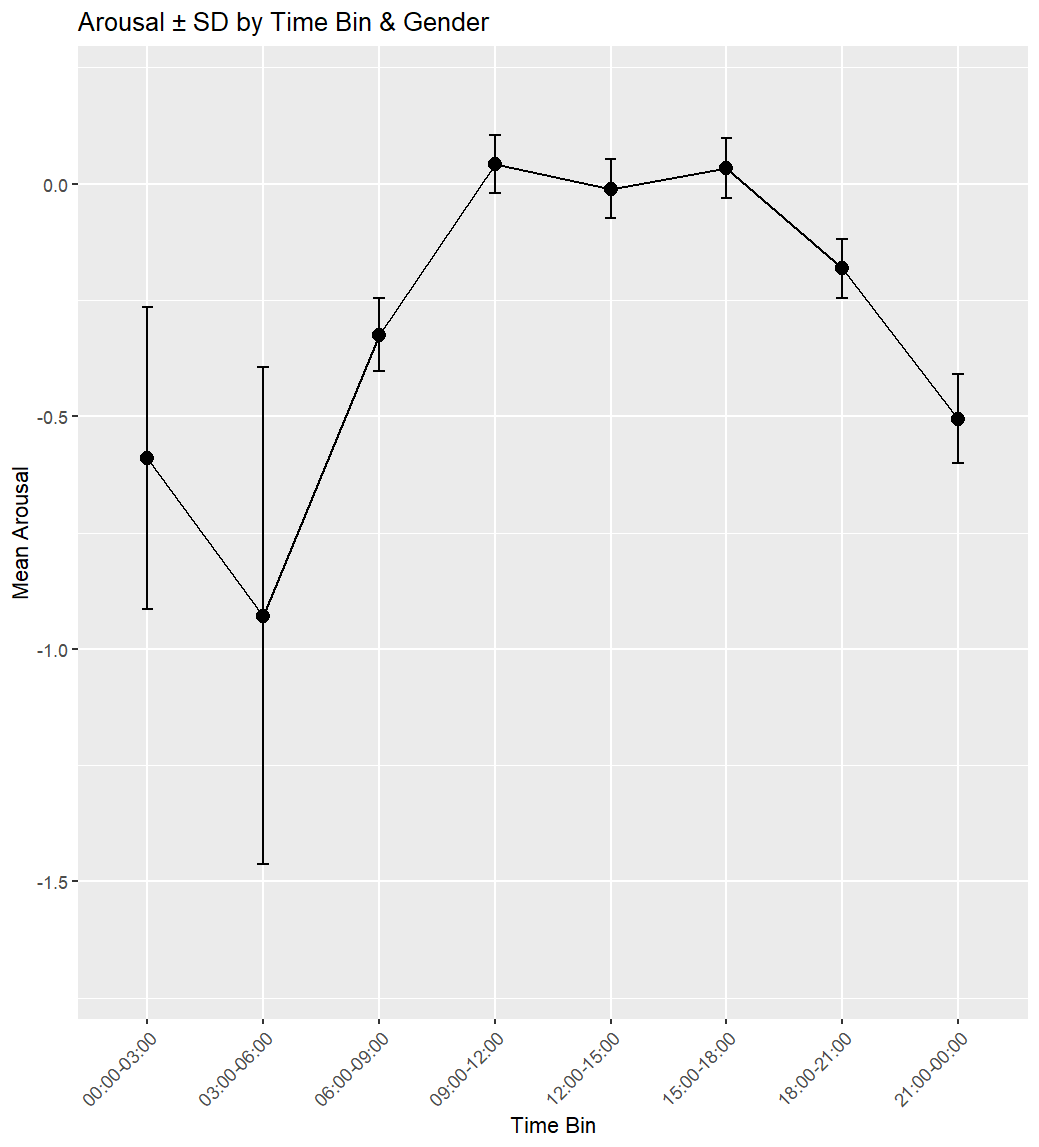
\includegraphics[width=\columnwidth]{/home/mori/projects/affective-forecast/R-workspace/arousal_by_timebin_and_gender.png}
     \caption{性別を考慮したArousal の推定平均値}
  \end{minipage}
%
  \begin{minipage}{0.4\columnwidth}
     \centering
     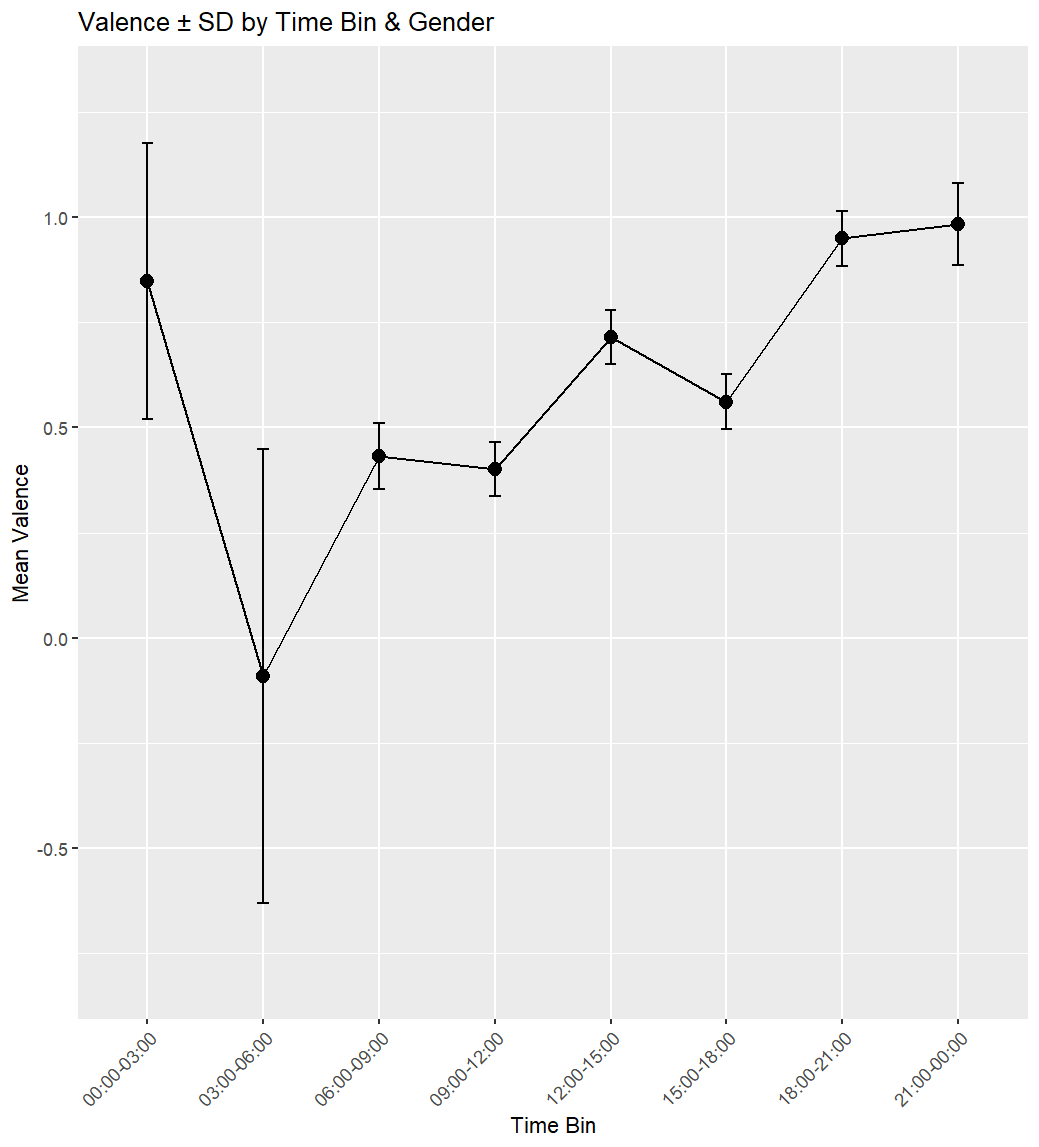
\includegraphics[width=\columnwidth]{/home/mori/projects/affective-forecast/R-workspace/valence_by_timebin_and_gender.png}
     \caption{性別を考慮したValence の推定平均値}
  \end{minipage}
\end{figure}

\vspace{3ex}
\subsubsection*{年齢による効果}
\begin{figure}[H]
  \centering
  \begin{minipage}{0.4\columnwidth}
     \centering
     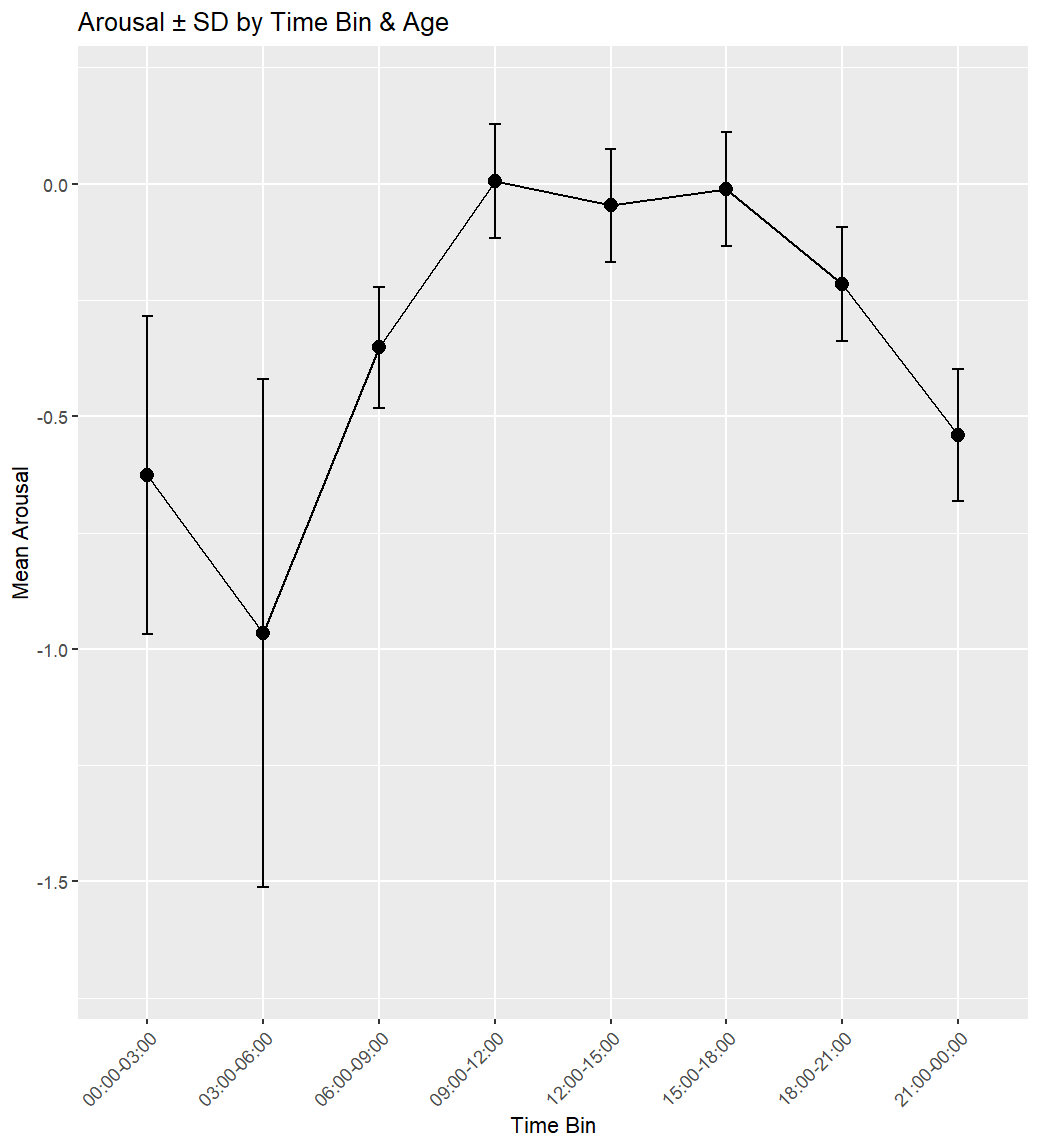
\includegraphics[width=\columnwidth]{/home/mori/projects/affective-forecast/R-workspace/arousal_by_timebin_and_age.png}
     \caption{年齢を考慮したArousal の推定平均値}
  \end{minipage}
%
  \begin{minipage}{0.4\columnwidth}
     \centering
     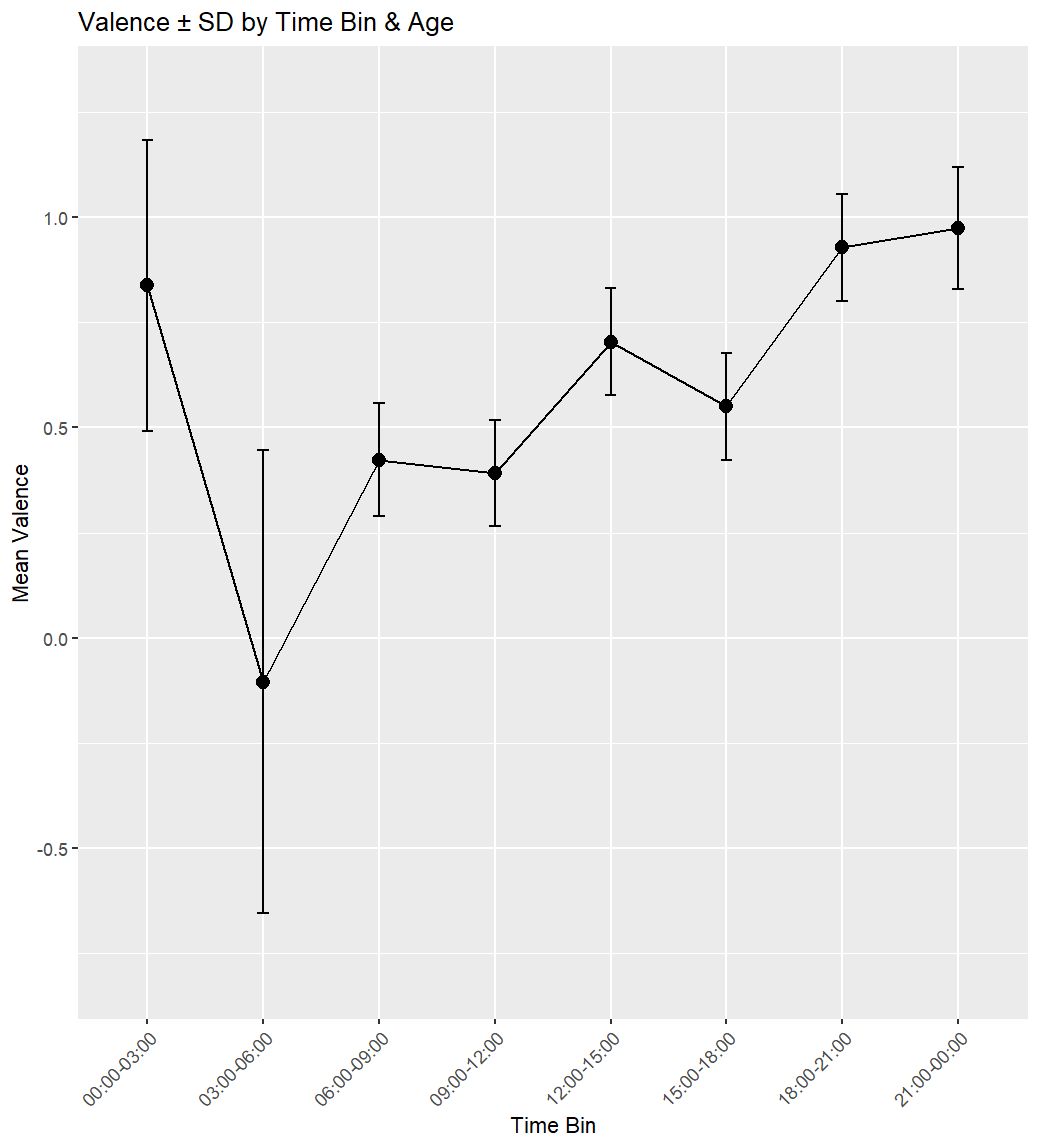
\includegraphics[width=\columnwidth]{/home/mori/projects/affective-forecast/R-workspace/valence_by_timebin_and_age.png}
     \caption{年齢を考慮したValence の推定平均値}
  \end{minipage}
\end{figure}

\vspace{3ex}
\subsubsection*{楽観性による効果}
\begin{figure}[H]
  \centering
  \begin{minipage}{0.4\columnwidth}
     \centering
     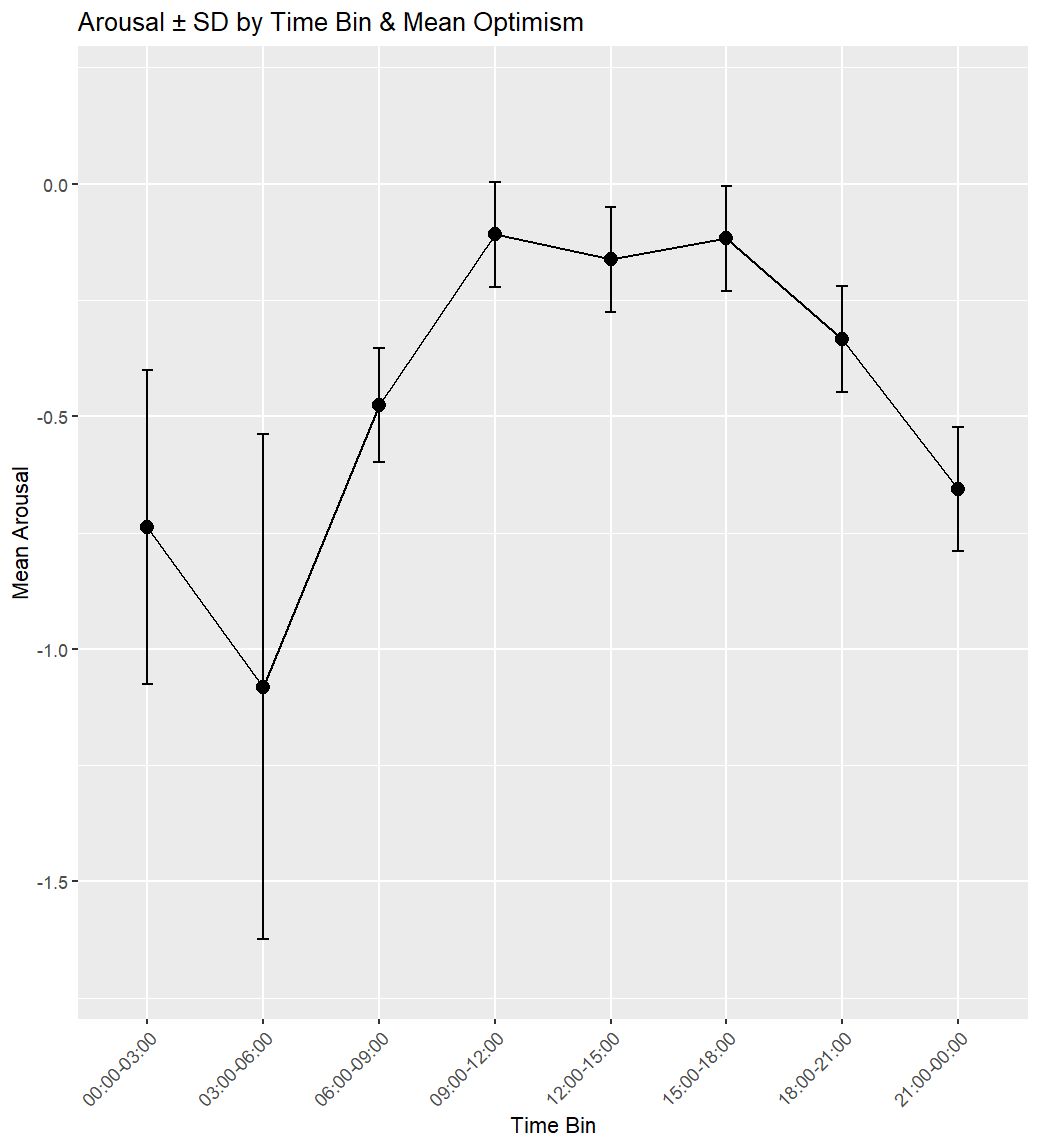
\includegraphics[width=\columnwidth]{/home/mori/projects/affective-forecast/R-workspace/arousal_by_timebin_and_meanoptimism.png}
     \caption{楽観性を考慮したArousal の推定平均値}
  \end{minipage}
%
  \begin{minipage}{0.4\columnwidth}
     \centering
     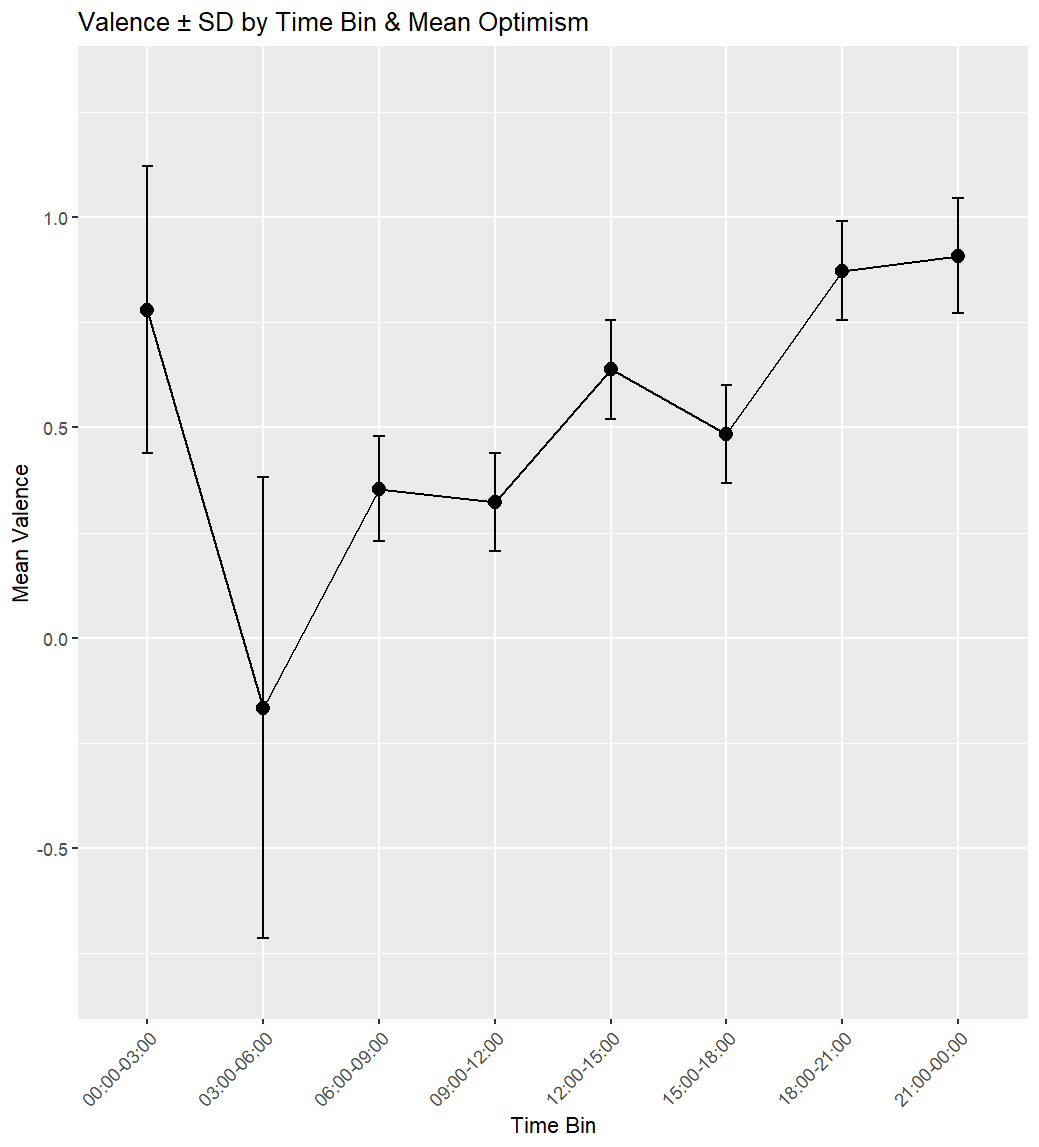
\includegraphics[width=\columnwidth]{/home/mori/projects/affective-forecast/R-workspace/valence_by_timebin_and_meanoptimism.png}
     \caption{楽観性を考慮したValence の推定平均値}
  \end{minipage}
\end{figure}

\vspace{3ex}
\subsubsection*{悲観性による効果}
\begin{figure}[H]
  \centering
  \begin{minipage}{0.4\columnwidth}
     \centering
     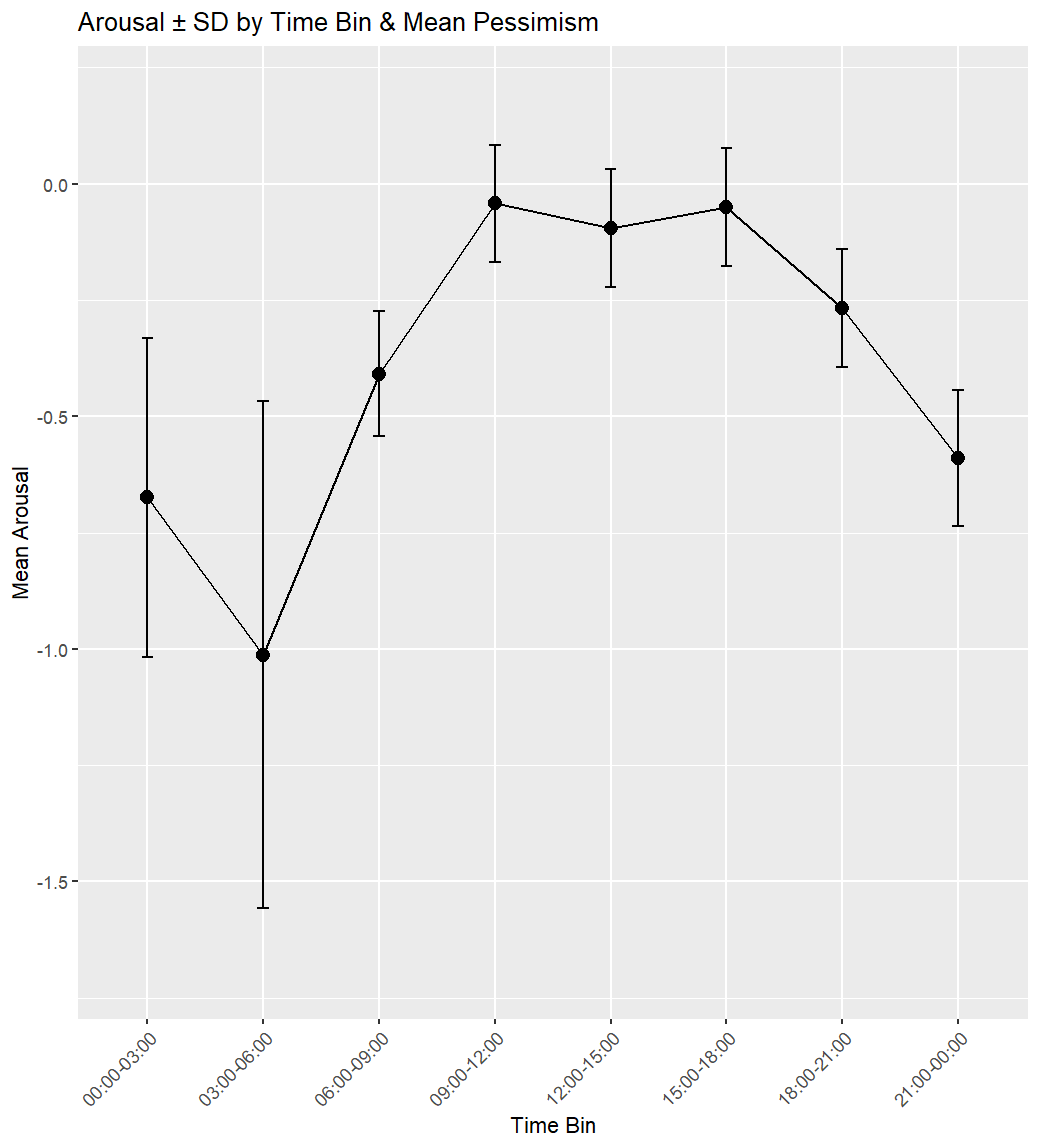
\includegraphics[width=\columnwidth]{/home/mori/projects/affective-forecast/R-workspace/arousal_by_timebin_and_meanpessimism.png}
     \caption{悲観性を考慮したArousal の推定平均値}
  \end{minipage}
%
  \begin{minipage}{0.4\columnwidth}
     \centering
     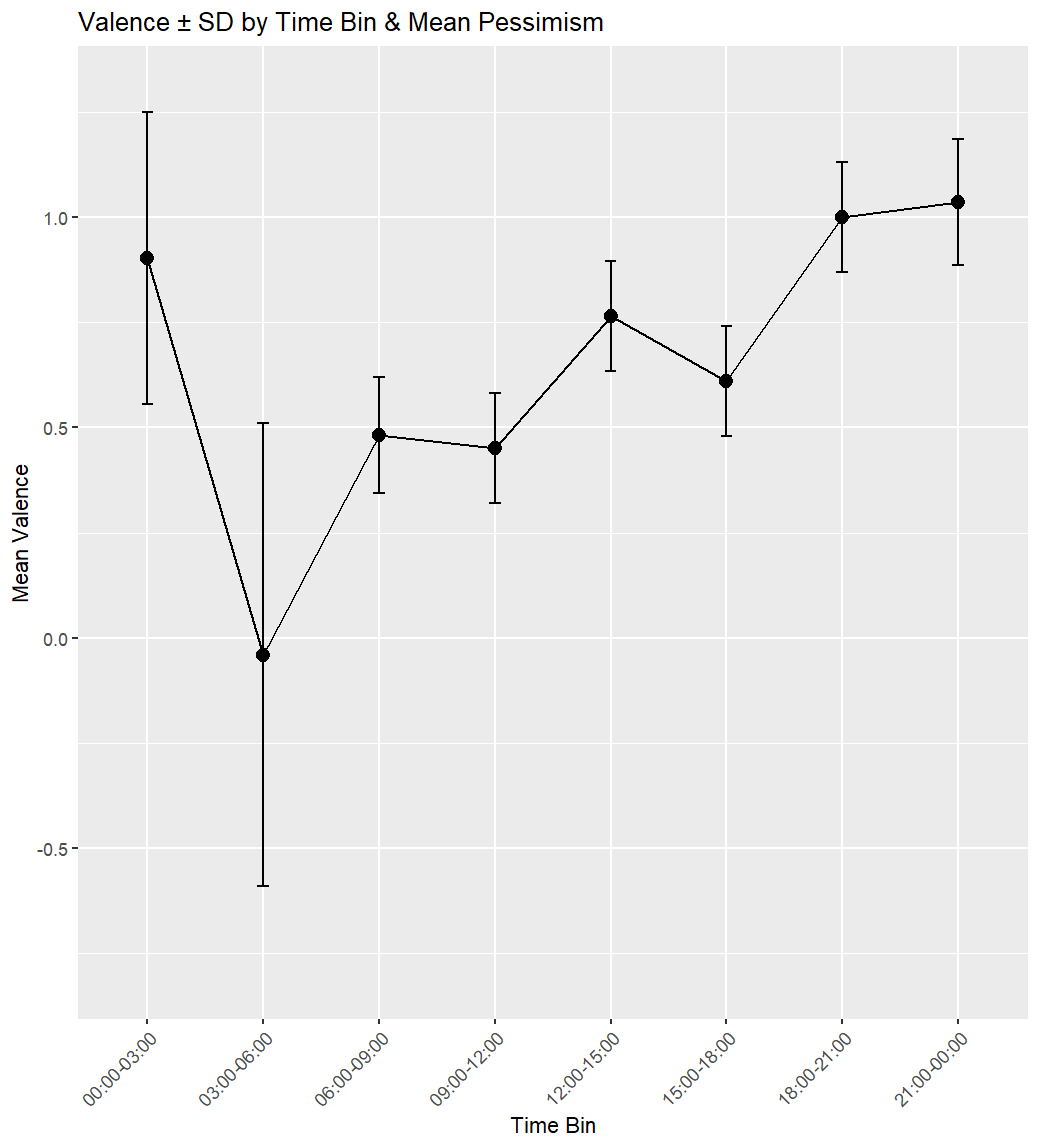
\includegraphics[width=\columnwidth]{/home/mori/projects/affective-forecast/R-workspace/valence_by_timebin_and_meanpessimism.png}
     \caption{悲観性を考慮したValence の推定平均値}
  \end{minipage}
\end{figure}


\subsection*{各時間帯ペアで推定平均値に有意な差があるかを検定}
Kenward–Roger(KR)法で補正をかけた後、t検定によって有意な差があるかどうかを検定


\end{document}


Linear mixed model fit by REML. t-tests use Satterthwaite's method ['lmerModLmerTest']
Formula: arousal ~ time_bin + (1 | subject_id)
   Data: dat

REML criterion at convergence: 115607

Scaled residuals: 
    Min      1Q  Median      3Q     Max 
-3.0746 -0.7178  0.0123  0.6870  3.5716 

Random effects:
 Groups     Name        Variance Std.Dev.
 subject_id (Intercept) 0.5818   0.7628  
 Residual               3.0672   1.7513  
Number of obs: 29057, groups:  subject_id, 164

Fixed effects:
                      Estimate Std. Error         df t value Pr(>|t|)  
(Intercept)         -5.895e-01  3.249e-01  2.483e+04  -1.814   0.0696 .
time_bin03:00-06:00 -3.398e-01  6.197e-01  2.892e+04  -0.548   0.5835  
time_bin06:00-09:00  2.647e-01  3.236e-01  2.897e+04   0.818   0.4134  
time_bin09:00-12:00  6.316e-01  3.202e-01  2.897e+04   1.972   0.0486 *
time_bin12:00-15:00  5.780e-01  3.204e-01  2.897e+04   1.804   0.0712 .
time_bin15:00-18:00  6.228e-01  3.204e-01  2.897e+04   1.944   0.0519 .
time_bin18:00-21:00  4.069e-01  3.204e-01  2.897e+04   1.270   0.2041  
time_bin21:00-00:00  8.392e-02  3.266e-01  2.894e+04   0.257   0.7972  
---
Signif. codes:  0 ‘***’ 0.001 ‘**’ 0.01 ‘*’ 0.05 ‘.’ 0.1 ‘ ’ 1

Correlation of Fixed Effects:
            (Intr) t_03:0 t_06:0 t_09:0 t_12:0 t_15:0 t_18:0
t_03:00-06: -0.507                                          
t_06:00-09: -0.971  0.511                                   
t_09:00-12: -0.981  0.515  0.986                            
t_12:00-15: -0.981  0.515  0.986  0.996                     
t_15:00-18: -0.981  0.515  0.986  0.996  0.995              
t_18:00-21: -0.980  0.515  0.985  0.996  0.995  0.995       
t_21:00-00: -0.957  0.502  0.962  0.972  0.971  0.971  0.971
> summary(valence_model)
Linear mixed model fit by REML. t-tests use Satterthwaite's method ['lmerModLmerTest']
Formula: valence ~ time_bin + (1 | subject_id)
   Data: dat

REML criterion at convergence: 116113.1

Scaled residuals: 
    Min      1Q  Median      3Q     Max 
-3.7348 -0.6254  0.1397  0.7133  3.2033 

Random effects:
 Groups     Name        Variance Std.Dev.
 subject_id (Intercept) 0.6284   0.7927  
 Residual               3.1200   1.7664  
Number of obs: 29057, groups:  subject_id, 164

Fixed effects:
                      Estimate Std. Error         df t value Pr(>|t|)   
(Intercept)             0.8537     0.3281 24358.8933   2.602  0.00927 **
time_bin03:00-06:00    -0.9399     0.6251 28917.2749  -1.504  0.13267   
time_bin06:00-09:00    -0.4186     0.3264 28964.1980  -1.283  0.19966   
time_bin09:00-12:00    -0.4499     0.3230 28962.0879  -1.393  0.16365   
time_bin12:00-15:00    -0.1359     0.3231 28962.2146  -0.421  0.67410   
time_bin15:00-18:00    -0.2898     0.3231 28962.0482  -0.897  0.36972   
time_bin18:00-21:00     0.0985     0.3232 28961.9745   0.305  0.76053   
time_bin21:00-00:00     0.1336     0.3294 28941.4941   0.406  0.68502   
---
Signif. codes:  0 ‘***’ 0.001 ‘**’ 0.01 ‘*’ 0.05 ‘.’ 0.1 ‘ ’ 1

Correlation of Fixed Effects:
            (Intr) t_03:0 t_06:0 t_09:0 t_12:0 t_15:0 t_18:0
t_03:00-06: -0.507                                          
t_06:00-09: -0.970  0.511                                   
t_09:00-12: -0.980  0.515  0.986                            
t_12:00-15: -0.980  0.515  0.986  0.996                     
t_15:00-18: -0.980  0.515  0.986  0.996  0.995              
t_18:00-21: -0.979  0.515  0.985  0.996  0.995  0.995       
t_21:00-00: -0.956  0.502  0.962  0.972  0.971  0.971  0.971
> 
> print(diffs_ar)
Least Squares Means table:

                                            Estimate Std. Error    df t value      lower      upper  Pr(>|t|)    
time_bin00:00-03:00 - time_bin03:00-06:00  0.3398163  0.6197361 28920  0.5483 -0.8748950  1.5545276  0.583474    
time_bin00:00-03:00 - time_bin06:00-09:00 -0.2646738  0.3236189 28969 -0.8179 -0.8989817  0.3696341  0.413446    
time_bin00:00-03:00 - time_bin09:00-12:00 -0.6315654  0.3201976 28966 -1.9724 -1.2591675 -0.0039634  0.048571 *  
time_bin00:00-03:00 - time_bin12:00-15:00 -0.5780378  0.3203519 28967 -1.8044 -1.2059422  0.0498667  0.071182 .  
time_bin00:00-03:00 - time_bin15:00-18:00 -0.6227823  0.3203620 28966 -1.9440 -1.2507065  0.0051419  0.051906 .  
time_bin00:00-03:00 - time_bin18:00-21:00 -0.4069149  0.3204077 28966 -1.2700 -1.0349287  0.2210990  0.204098    
time_bin00:00-03:00 - time_bin21:00-00:00 -0.0839161  0.3265594 28945 -0.2570 -0.7239875  0.5561553  0.797203    
time_bin03:00-06:00 - time_bin06:00-09:00 -0.6044901  0.5327302 28898 -1.1347 -1.6486658  0.4396856  0.256510    
time_bin03:00-06:00 - time_bin09:00-12:00 -0.9713817  0.5311624 28899 -1.8288 -2.0124846  0.0697211  0.067442 .  
time_bin03:00-06:00 - time_bin12:00-15:00 -0.9178541  0.5312312 28899 -1.7278 -1.9590917  0.1233835  0.084037 .  
time_bin03:00-06:00 - time_bin15:00-18:00 -0.9625986  0.5312400 28899 -1.8120 -2.0038535  0.0786564  0.069999 .  
time_bin03:00-06:00 - time_bin18:00-21:00 -0.7467311  0.5312841 28899 -1.4055 -1.7880725  0.2946102  0.159877    
time_bin03:00-06:00 - time_bin21:00-00:00 -0.4237324  0.5360427 28902 -0.7905 -1.4744008  0.6269360  0.429253    
time_bin06:00-09:00 - time_bin09:00-12:00 -0.3668916  0.0538085 28970 -6.8185 -0.4723587 -0.2614246 9.382e-12 ***
time_bin06:00-09:00 - time_bin12:00-15:00 -0.3133640  0.0545474 28964 -5.7448 -0.4202793 -0.2064487 9.295e-09 ***
time_bin06:00-09:00 - time_bin15:00-18:00 -0.3581085  0.0546319 28964 -6.5549 -0.4651895 -0.2510275 5.660e-11 ***
time_bin06:00-09:00 - time_bin18:00-21:00 -0.1422410  0.0549437 28964 -2.5889 -0.2499332 -0.0345489  0.009634 ** 
time_bin06:00-09:00 - time_bin21:00-00:00  0.1807577  0.0897842 28993  2.0132  0.0047766  0.3567389  0.044098 *  
time_bin09:00-12:00 - time_bin12:00-15:00  0.0535277  0.0292153 28912  1.8322 -0.0037357  0.1107911  0.066935 .  
time_bin09:00-12:00 - time_bin15:00-18:00  0.0087832  0.0293805 28912  0.2989 -0.0488039  0.0663703  0.764984    
time_bin09:00-12:00 - time_bin18:00-21:00  0.2246506  0.0299869 28911  7.4916  0.1658749  0.2834263 6.997e-14 ***
time_bin09:00-12:00 - time_bin21:00-00:00  0.5476494  0.0772256 28996  7.0915  0.3962836  0.6990151 1.357e-12 ***
time_bin12:00-15:00 - time_bin15:00-18:00 -0.0447445  0.0308083 28900 -1.4524 -0.1051302  0.0156412  0.146415    
time_bin12:00-15:00 - time_bin18:00-21:00  0.1711229  0.0314009 28902  5.4496  0.1095757  0.2326702 5.089e-08 ***
time_bin12:00-15:00 - time_bin21:00-00:00  0.4941217  0.0777906 28995  6.3519  0.3416485  0.6465949 2.158e-10 ***
time_bin15:00-18:00 - time_bin18:00-21:00  0.2158674  0.0315560 28900  6.8408  0.1540162  0.2777187 8.034e-12 ***
time_bin15:00-18:00 - time_bin21:00-00:00  0.5388662  0.0778124 28993  6.9252  0.3863502  0.6913821 4.445e-12 ***
time_bin18:00-21:00 - time_bin21:00-00:00  0.3229988  0.0779623 28992  4.1430  0.1701890  0.4758085 3.437e-05 ***
---
Signif. codes:  0 ‘***’ 0.001 ‘**’ 0.01 ‘*’ 0.05 ‘.’ 0.1 ‘ ’ 1

  Confidence level: 95%
  Degrees of freedom method: Kenward-Roger 
> print(diffs_va)
Least Squares Means table:

                                           Estimate Std. Error    df  t value     lower     upper  Pr(>|t|)    
time_bin00:00-03:00 - time_bin03:00-06:00  0.939918   0.625067 28918   1.5037 -0.285243  2.165079 0.1326679    
time_bin00:00-03:00 - time_bin06:00-09:00  0.418628   0.326412 28965   1.2825 -0.221155  1.058411 0.1996728    
time_bin00:00-03:00 - time_bin09:00-12:00  0.449859   0.322961 28963   1.3929 -0.183159  1.082877 0.1636545    
time_bin00:00-03:00 - time_bin12:00-15:00  0.135877   0.323117 28963   0.4205 -0.497446  0.769201 0.6741083    
time_bin00:00-03:00 - time_bin15:00-18:00  0.289840   0.323127 28963   0.8970 -0.343503  0.923184 0.3697334    
time_bin00:00-03:00 - time_bin18:00-21:00 -0.098498   0.323173 28963  -0.3048 -0.731932  0.534936 0.7605327    
time_bin00:00-03:00 - time_bin21:00-00:00 -0.133602   0.329373 28942  -0.4056 -0.779188  0.511985 0.6850219    
time_bin03:00-06:00 - time_bin06:00-09:00 -0.521290   0.537307 28897  -0.9702 -1.574436  0.531857 0.3319600    
time_bin03:00-06:00 - time_bin09:00-12:00 -0.490059   0.535726 28898  -0.9148 -1.540106  0.559989 0.3603271    
time_bin03:00-06:00 - time_bin12:00-15:00 -0.804041   0.535795 28898  -1.5006 -1.854224  0.246143 0.1334573    
time_bin03:00-06:00 - time_bin15:00-18:00 -0.650077   0.535804 28898  -1.2133 -1.700278  0.400124 0.2250350    
time_bin03:00-06:00 - time_bin18:00-21:00 -1.038416   0.535849 28898  -1.9379 -2.088704  0.011872 0.0526464 .  
time_bin03:00-06:00 - time_bin21:00-00:00 -1.073520   0.540649 28901  -1.9856 -2.133216 -0.013823 0.0470857 *  
time_bin06:00-09:00 - time_bin09:00-12:00  0.031231   0.054273 28966   0.5754 -0.075147  0.137608 0.5649986    
time_bin06:00-09:00 - time_bin12:00-15:00 -0.282751   0.055018 28960  -5.1392 -0.390589 -0.174913 2.776e-07 ***
time_bin06:00-09:00 - time_bin15:00-18:00 -0.128788   0.055103 28961  -2.3372 -0.236793 -0.020783 0.0194352 *  
time_bin06:00-09:00 - time_bin18:00-21:00 -0.517126   0.055418 28961  -9.3314 -0.625748 -0.408505 < 2.2e-16 ***
time_bin06:00-09:00 - time_bin21:00-00:00 -0.552230   0.090561 28989  -6.0979 -0.729733 -0.374727 1.088e-09 ***
time_bin09:00-12:00 - time_bin12:00-15:00 -0.313982   0.029467 28911 -10.6555 -0.371738 -0.256226 < 2.2e-16 ***
time_bin09:00-12:00 - time_bin15:00-18:00 -0.160019   0.029633 28911  -5.4000 -0.218101 -0.101936 6.717e-08 ***
time_bin09:00-12:00 - time_bin18:00-21:00 -0.548357   0.030245 28910 -18.1307 -0.607638 -0.489076 < 2.2e-16 ***
time_bin09:00-12:00 - time_bin21:00-00:00 -0.583461   0.077894 28992  -7.4905 -0.736136 -0.430785 7.058e-14 ***
time_bin12:00-15:00 - time_bin15:00-18:00  0.153963   0.031073 28899   4.9549  0.093059  0.214868 7.278e-07 ***
time_bin12:00-15:00 - time_bin18:00-21:00 -0.234375   0.031671 28901  -7.4004 -0.296451 -0.172299 1.395e-13 ***
time_bin12:00-15:00 - time_bin21:00-00:00 -0.269479   0.078464 28990  -3.4344 -0.423271 -0.115687 0.0005946 ***
time_bin15:00-18:00 - time_bin18:00-21:00 -0.388338   0.031827 28899 -12.2015 -0.450721 -0.325956 < 2.2e-16 ***
time_bin15:00-18:00 - time_bin21:00-00:00 -0.423442   0.078486 28989  -5.3952 -0.577277 -0.269607 6.900e-08 ***
time_bin18:00-21:00 - time_bin21:00-00:00 -0.035104   0.078637 28987  -0.4464 -0.189235  0.119028 0.6553086    
---
Signif. codes:  0 ‘***’ 0.001 ‘**’ 0.01 ‘*’ 0.05 ‘.’ 0.1 ‘ ’ 1

  Confidence level: 95%
  Degrees of freedom method: Kenward-Roger 